\subsection{Linear Blend Skinning}

Linear Blend Skinning ist der am weiten verbreitetste Skinning-Algorithmus, vermutlich auf Grund seiner geringen Kosten \cite{kavan2008geometric}. Er wurde zuerst hier \cite{lewis2000pose} beschrieben. Um Linear Blend Skinning zu verstehen, m�ssen wir die bisher erarbeiteten Konzepte kombinieren. Wir beziehen in unsere direkte Skinning-Formel die Transformation jedes Knochen mit ein und modifizieren sie durch das Gewicht in Relation zu diesem Knochen. So wird die Transformation von Punkten mit Gewicht 0 ignoriert, bei einem Gewicht von 1 voll einbezogen und dazwischen teilweise ber�cksichtigt.

\begin{equation}
\label{formel}
v'=\sum_{i=1}^{N}w_{i}W_{ji}(v)
\end{equation}

\begin{figure}[t]
	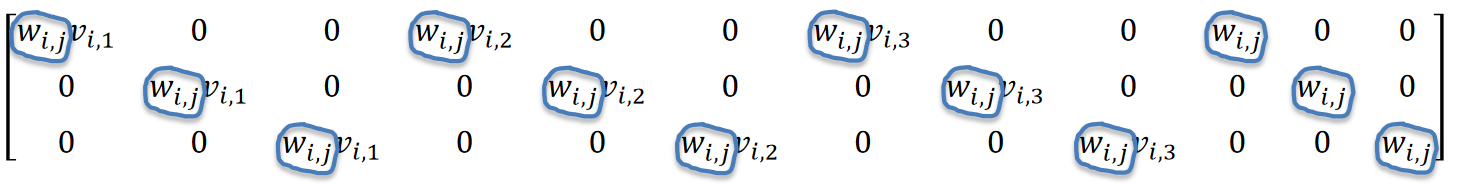
\includegraphics[width=11cm]{01_Skinning/pics/lbsmatrix.png}
	\caption[Darstellung Linear Blend Skinning als Matrix-Multiplikation]{Matrix Multiplikation bei Linear Blend Skinning.  Entnommen von \cite{skinningcourse:2014}}
	\label{lbsMatrix_fig1}
\end{figure}

Am besten ist dies zu verstehen, indem man die Matrix auf Abbildung 11. betrachtet. Hier wird sehr deutlich, dass es durch Multiplikation der Transformations-Matrix mit $v_{i}$, immer nur ein Gewicht-Knochen Paar gibt.  

Dieser Algorithmus kommt auch Animationsfilmen, die es bis in die Kinos schaffen, zum Einsatz. Das einzige Problem dieses Algorithmus ist jedoch, dass er sich in der euklidischen Geometrie bewegt und damit Volumenverlusten und andere Artefakte m�glich macht. Sehr eindrucksvoll l�sst sich dies an einem einfachen Beispiel in Abbildung 12 illustrieren. Nehmen wir an, wir h�tten ein einfaches Gelenk mit zwei Knochen $j_{1}$ und $j_{2}$. Punkt $v$ ist gleicherma�en mit einem Gewicht von 0.5 an sowohl $j_{1}$ als auch $j_{2}$ gebunden. Nun geschieht an $j2$ eine Drehung von 180�. Wie man in folgender Grafik gut erkennen kann landet $v$ genau auf dem Knochen und damit kollabiert die Haut auf einen Punkt. 

\begin{figure}[t]
	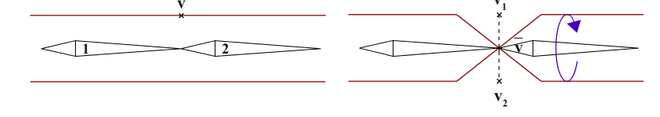
\includegraphics[width=11cm]{01_Skinning/pics/rotationsartefakt.png}
	\caption[Volumenverlust bei Rotation in LBS]{Darstellung des Volumenverlust bei Linear Blend Skinning. Da die beiden Punkte mit gleichen Gewicht an beiden Knochen h�ngen reduzieren sie sich auf einen Punkt. Entnommen von \cite{weights}}
	\label{weights_fig1}
\end{figure}